
%(BEGIN_QUESTION)
% Copyright 2006, Tony R. Kuphaldt, released under the Creative Commons Attribution License (v 1.0)
% This means you may do almost anything with this work of mine, so long as you give me proper credit

En svært vanlig metode for å regulere ``strømningen'' av pulver eller granulert faststoff inn i en prosess er en mekanisme med variabel hastighet på transportbånd og vekt, kalt {\it weighfeeder} eller {\it gravimetric belt feeder}. En mulig bruk av en slik enhet er dosering av kullpulver inn i en ovn eller en stor dampkjel for kraftproduksjon:

$$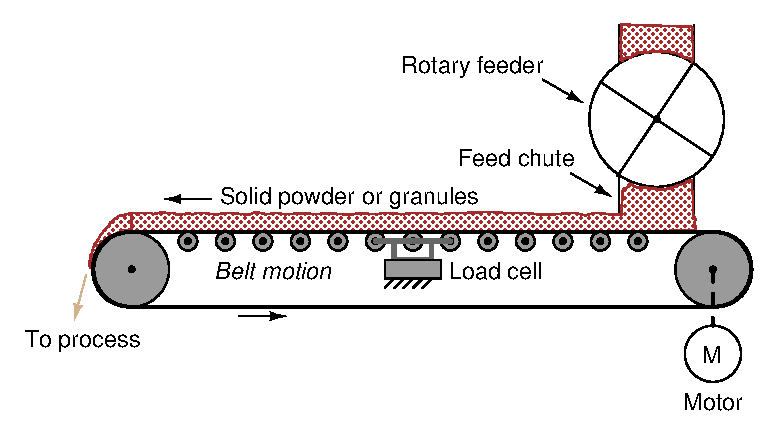
\includegraphics[width=15.5cm]{i01431x01.eps}$$

I illustrasjonen over er en kort seksjon av båndet støttet av et sett ruller koblet til en lastcelle. Dette gir i praksis veiing av en seksjon av lastet bånd. Hvis vi vet lengden på denne rulleseksjonen, kan vektverdien i pund omregnes til pund per fot (av bånd). Alt vi trenger i tillegg er båndhastigheten, så kan vi beregne pund per minutt materiale levert til prosessen.

Forklar hvordan en elektrisk motor med variabel hastighet er avgjørende for å kunne regulere mengden faststoff som går til prosessen. Identifiser også hvilke enheter som må {\it låses ut} av sikkerhetshensyn før mekanisk vedlikeholdsarbeid utføres på systemet.

\vskip 20pt \vbox{\hrule \hbox{\strut \vrule{} {\bf Forslag til sokratisk diskusjon} \vrule} \hrule}

\begin{itemize}
\item{} Hvis du fikk i oppgave å programmere en PLS for å beregne massestrøm i sanntid over denne weighfeederen, hvordan ville du gjort det (i grove trekk)? Hvilke sensorer måtte du installere? Hvor mange analoge inngangskanaler måtte PLS-en ha? Hvilken type beregning(er) måtte PLS-en utføre på signalene?
\end{itemize}

\underbar{file i01431}
%(END_QUESTION)





%(BEGIN_ANSWER)

Vanligvis er båndets drivmotor variabel i hastighet, og det samme gjelder motoren som driver den roterende materen.

%(END_ANSWER)





%(BEGIN_NOTES)

%INDEX% Final Control Elements, motor: weighfeeder

%(END_NOTES)

